\documentclass[11pt, oneside]{article}   	% use "amsart" instead of "article" for AMSLaTeX format
\usepackage{geometry}                		% See geometry.pdf to learn the layout options. There are lots.
\geometry{letterpaper}                   		% ... or a4paper or a5paper or ... 
%\geometry{landscape}                		% Activate for for rotated page geometry
%\usepackage[parfill]{parskip}    		% Activate to begin paragraphs with an empty line rather than an indent
\usepackage{graphicx}				% Use pdf, png, jpg, or eps� with pdflatex; use eps in DVI mode
								% TeX will automatically convert eps --> pdf in pdflatex		
\usepackage{amssymb}
\usepackage{amsmath}
\usepackage{parskip}
\usepackage{color}
\usepackage{hyperref}

\title{Cauchy integral theorem}
%\author{The Author}
%\section{}
%\subsection*{}
\date{}							% Activate to display a given date or no date

\graphicspath{{/Users/telliott_admin/Dropbox/Tex/png/}}
% \begin{center} 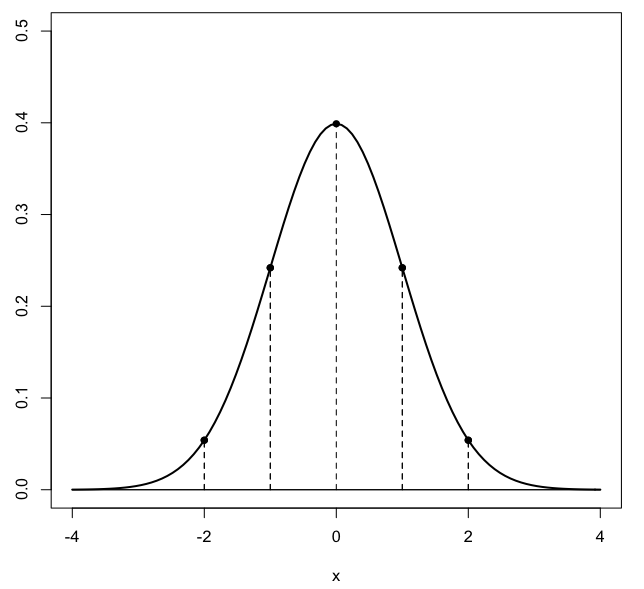
\includegraphics [scale=0.4] {gauss3.png} \end{center}
\begin{document}
\maketitle
\Large

\subsection*{derivation of Cauchy 2}
Suppose $f(z)$ is analytic everywhere within some region \emph{except} at a singularity, $z_0$.  For example, suppose we have
\[ \frac{f(z)}{z-z_0} \]
and suppose we integrate this around a special closed path in the region of analyticity:
\[ \oint \frac{f(z)}{z-z_0} \ dz \]
\begin{center} 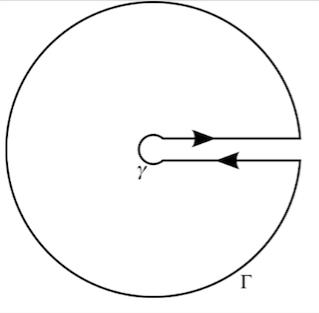
\includegraphics [scale=0.6] {keyhole.png} \end{center}
It's not labeled but the singularity $z_0$ is at the center of the two concentric circles.  The "keyhole" excludes $z_0$ so $f$ is analytic everywhere in the region enclosed by the path, and the total integral is zero by Cauchy's first theorem.  The straight line segments are so close as to be equal, but traversed in opposite directions, so the contribution from them is zero.  Thus we have that the integral around the outer ring counter-clockwise + the integral around the inner ring clockwise add up to zero.

Reversing the direction of integration on the inner ring changes the sign of the value, hence we have that
\[ \oint_{C \ \text{outer}} \frac{f(z)}{z-z_0} \ dz - \oint_{C \ \text{inner}} \frac{f(z)}{z-z_0} \ dz = 0 \]
But we haven't said anything about the radius of these rings.  

What this means is that the value of the integral around a ring enclosing a singularity is not zero, but it has the same value for a ring of \emph{any} radius.  It's independent of the radius.
\[ \oint_{C \ \text{outer}} \frac{f(z)}{z-z_0} \ dz = \oint_{C \ \text{inner}} \frac{f(z)}{z-z_0} \ dz \]

We can parametrize this path by saying that each point on the curve is given by
\[ z = z_0 + \rho e^{i\theta}, \ \ \ 0 \le \theta \le 2 \pi \]
\[ dz = \rho i e^{i \theta} \ d \theta \]
\[ \oint \frac{f(z)}{z - z_0} \ dz = \int_0^{2\pi} \frac{f(z_0 + \rho e^{i\theta})}{\rho e^{i \theta}} \ \rho i e^{i\theta} \ d \theta \]
\[ = i \int_0^{2\pi}  f(z_0 + \rho e^{i\theta}) \ d \theta \]
\[ = i \int_0^{2\pi}  f(z) \ d \theta \]
We may choose $\rho$ as small as we like, and in particular, if we choose it very small ($\rho \rightarrow 0$) we have
\[ f(z) \rightarrow f(z_0) = \text{constant} \]
and since it's constant we can bring it out of the integral!
\[  \oint \frac{f(z)}{z - z_0} \ dz = f(z_0) i \int_0^{2\pi} d \theta \]
\[ = 2 \pi i f(z_0) \]

\subsection*{example}
We can use the inverse function ($1/z$) as an example.  This function has a singularity at the origin.  Compare with the form of Cauchy2:
\[  \oint \frac{f(z)}{z - z_0} \ dz = f(z_0) i \int_0^{2\pi} d \theta = 2 \pi i f(z_0) \]
We match this form if we set $f(z) = 1$ and $z_0 = 0$.  The theorem says we can write the value of the integral as
\[ I = 2 \pi i f(z_0) = 2 \pi i \]
This matches what we obtained by parametrizing the unit circle.  Then we had
\[ z = e^{i\theta}, \ \ \ \theta = 0 \rightarrow 2 \pi \]
\[ \frac{dz}{d \theta} = iz \]
\[ \oint \frac{dz}{z} = \int_0^{2\pi} i \ d \theta = 2 \pi i \]

\end{document}  
